\documentclass[10pt]{beamer}
\usepackage{xeCJK}
\usepackage{listings}
\usepackage{tikz}
\usepackage{subfigure}
\usepackage{color}
\usepackage[ruled,linesnumbered,titlenotnumbered,noend,vlined]{algorithm2e}
\usetikzlibrary{arrows,automata}

\renewcommand{\thealgocf}{}

\usetheme[
%	sidebar, % 默认不显示包含幻灯片结构的边框。如设置sidebar选项,则参考AAU模板显示左边框
	footline,
	blue, % 主色调默认为红色,色调可以选择red和blue
%	wide, % 幻灯片的长宽比默认为4:3,如设置了wide选项则为16:9
	hideallsubsections, % 默认显示所有等级的标题。如设置了hideallsubsections,
	                    % 则不显示小节标题
	mathserif, % 默认公式字体是钝化的,如设置mathserif选项则采用正常的公式字体
%	english, % 默认幻灯片环境为中文,如设置english选项则采用英文的章节和图表编号
	sectiontoc, % 设置sectiontoc选项则在每节(section)之前添加一个所有节的目录,
	            % 并标明本节在整个幻灯片中的位置,不建议和\part层级一同使用
]{SEUstyle}

\title[第四组报告]{强化学习与规划 \\ 强化学习在游戏中的应用}
\author[张舒韬 et al.]{刘翔~吴江恒~张舒韬~赵倩隆}
\institute[SEU CS Dept. Team 4]{东南大学\ 计算机科学与工程学院\ 第4组}

\begin{document}
	{\background
		\begin{frame}[plain,noframenumbering]
			\titlepage
		\end{frame}
	}

	\begin{frame}{总目录}
		第I部分 强化学习与规划
		\tableofcontents[part=1]
		第II部分 强化学习在FPS游戏中的应用
		\tableofcontents[part=2]
	\end{frame}

	\part{强化学习与规划}\label{part:rl-and-planning}
	
	\section{背景知识回顾}
	
	\subsection{马尔科夫决策过程}
	
	\begin{frame}{马尔科夫决策过程}{定义}
		\visible<1->{
			一个马尔科夫决策过程是一个五元组$D = \langle S,A,P,r,\gamma \rangle$,其中
			\begin{description}
				\item[$S$] 过程中的状态(state)集合
				\item[$A$] 过程中的动作(action)集合
				\item[$P$] 转移函数(transition function)$P(s, a, s')$定义为$S \times A \times S \rightarrow [0,1]$,表示在状态$s$时选择动作$a$达到状态$s'$的概率
				\item[$r$] 奖励函数(reward function)$r(s, a, s')$定义为$S \times A \times S \rightarrow \mathbb{R}$,表示在状态$s$时选择动作$a$达到状态$s'$时得到的奖励
				\item[$\gamma$] 折扣因子(discount factor)$\gamma \in [0,1]$
			\end{description}
		}
		
		\visible<2->{
			累积奖励的定义
			\begin{equation*}
			\sum^{\infty}_{t=0} {\gamma^t r(s_t, a_t, s_{t+1})}   
			\end{equation*}
		}
	\end{frame}

	\begin{frame}{马尔科夫决策过程}{问题}
		\begin{description}
			\item<2->[预测问题(Predicting)] 已知起始状态、转移函数和决策策略,求在此情况下能够得到的累积奖励的期望;
			\item<3->[规划问题(Planning)] 已知起始状态和转移函数,求使累积奖励的期望值最大的决策策略;
			\item<4->[强化学习(Reinforcement Learning)] 转移函数或奖励函数未知,求使累积奖励的期望值最大的决策策略。
		\end{description}
	\end{frame}

	\begin{frame}{马尔科夫决策过程}{规划与学习}
		\begin{figure}
			\centering
			\begin{tikzpicture}[->,>=stealth',shorten >=1pt,auto,node distance=30cm,semithick,bend angle=40]
			\tikzstyle{every state}=[rectangle,font=\bfseries,fill=white,draw=none,text=black]
			\node (policy) at (0,0)           [state] {value/policy};
			\node (exper)  at (1*2,-1.732*2)  [state] {experience};
			\visible<1,3>{\node (model)  at (-1*2,-1.732*2) [state] {model};}
			
			\path (policy) edge [bend left] node {acting} (exper);
			\visible<1-2>{\path (exper)  edge [bend left] node {direct RL} (policy);}
			\visible<1,3>{\path (exper) edge [bend left] node {model learning} (model);}
			\visible<1,3>{\path (model)  edge [bend left] node {planning} (policy);}
			
			\only<1>{\node at (0,-5.5) [state] { };}
			\only<2>{\node at (0,-5.5) [state,text=red] {Model-Free RL};}
			\only<3>{\node at (0,-5.5) [state,text=red] {Model-Based RL};}
			\end{tikzpicture}
			\caption{学习、规划和执行之间的关系\protect\cite{Sutton1998:RL-Introduction}}\label{fig:relation-in-RL}
		\end{figure}
	\end{frame}

	\subsection{Q-Learning}
	
	\begin{frame}{Q-Learning}{定义}
		\begin{itemize}
			\item<2-> Q-Learning是一种off-policy的时序差分学习方法
			\item<3-> Q-Learning的目标是得到$Q^*$函数的估计,即
			\[Q^*(s,a) = \max_{\pi}\mathbb{E}(R_t | s_t = t, a_t = a, \pi) \]
			\[Q^*(s,a) = \mathbb{E}\left[r_{t+1} + \gamma \max_{a' \in A(s)} Q^*(s_{t+1}, a') | s_t = s, a_t = a\right] \]
			\item<4-> Q-learning的定义为
			\[ Q(s_t, a_t) \gets Q(s_t, a_t) + \alpha \left[r_{t+1} + \gamma \max_{a \in A(s_{t+1})}Q(s_{t+1}, a) - Q(s_t, a_t) \right] \]
		\end{itemize}
	\end{frame}

	\begin{frame}{Q-Learning}{算法描述}
		\begin{algorithm}[H]
			随机初始化$Q(s, a)$\;
			\ForEach{每个周期(episode)}{
				初始化$s$\;
				\ForEach{周期内的每一步,直到$s$为终止状态}{
					利用$Q$函数中获得的策略(例如$\epsilon$-greedy)选择状态$s$时采取的策略\;
					执行$a$,观察$s'$和$r'$\;
					$Q(s_t, a_t) \gets Q(s_t, a_t) + \alpha [r_{t+1} + \gamma \max_{a}Q(s_{t+1}, a) - Q(s_t, a_t) ]$\;
				}
			}
			\caption{Q-Learning}\label{alg:q-learning}
		\end{algorithm}
	\end{frame}

	\begin{frame}{基于强化学习的规划}{Q-Planning}
		
		\begin{figure}
			\centering
			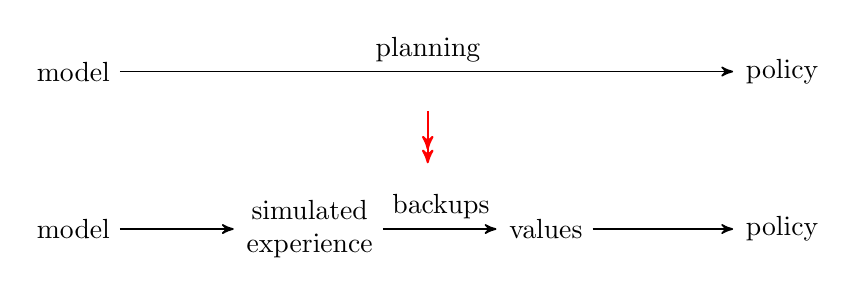
\begin{tikzpicture}[->,>=stealth',shorten >=1pt,auto,node distance=50cm,semithick]
			\tikzstyle{every state}=[rectangle,fill=white,draw=none,text=black,align=center]
				\visible<2->{
					\node (model0) at(0,2) [state] {model};
					\node (policy0) at(9,2) [state] {policy};
					
					\path (model0) edge node {planning} (policy0);
				}
			
				\visible<3-> {
					\draw [->>,thick,draw=red] (4.5,1.5) -- (4.5,0.8);
					\node (model) at(0,0) [state] {model};
					\node (exper) at(3,0) [state] {simulated\\ experience};
					\node (values) at(6,0) [state] {values};
					\node (policy) at(9,0) [state] {policy};
					
					\path (model) edge (exper)
					(exper) edge node {backups} (values)
					(values) edge (policy);
				}
			\end{tikzpicture}
		\end{figure}
	
		\visible<4->{
			\begin{algorithm}[H]
				\Repeat{stop}{
					随机选择$s \in S$, $a \in A(s)$\;
					根据模型模拟出下一状态$s'$和奖励$r$\;
					更新$Q(s,a) \gets Q(s,a) + \alpha[r + \gamma \max_{a'}Q(s',a') - Q(s,a)]$\;
				}
				\caption{随机Q-Planning}
			\end{algorithm}
		}
		
	\end{frame}

	\begin{frame}{强化学习}{强化学习的两种方法}
		\begin{small}		
			\begin{description}
				\item<2->[Model-Based RL] 
				
				优点:
				\begin{itemize}
					\item 有时直接从环境中学到值函数较难,而模型的$P(s’|s,a)$和$R(r|s,a)$很容易就能用监督学习去学;
				\end{itemize}
				
				缺点:
				\begin{itemize}
					\item 误差来源多了模型拟合的误差;
				\end{itemize}
				
				\item<3->[Model-Free RL] 优点:
				\begin{itemize}
					\item 不需要具体的环境模型;
					\item 使用时做出决策的时间快;
				\end{itemize}
				
				缺点:
				\begin{itemize}
					\item 优化过程可能不稳定且不收敛;
					\item 比较难适应变化的环境;
				\end{itemize}
			\end{description}
		\end{small}
	\end{frame}

	\begin{frame}{强化学习}{Model-Free or Model-Based?}
		All models are wrong, but some are useful.
		\begin{flushright}
			--George E.P. Box, Robustness in the strategy of scientific model building
		\end{flushright}
	
		\begin{figure}
			\centering
			\begin{tikzpicture}
				\visible<2->{\node at (0,0) {\includegraphics[width=.4\linewidth]{pictures/newton.png}};}
				\visible<3->{\node at(2,0) {\includegraphics[width=.5\linewidth]{pictures/einstein.png}};}
				\visible<4->{\node at(4,0) {\includegraphics[width=.4\linewidth]{pictures/cat.png}};}
			\end{tikzpicture}
		\end{figure}
	\end{frame}

	\section{两种规划与学习结合的方法}
	
	\subsection{Dyna}
	
	\begin{frame}{Dyna}{主要思想和结构}
		\begin{figure}
			\centering
			\includegraphics[width=0.6\linewidth]{pictures/dyna-arch.png}
			\caption{Dyna agent的一般结构}
			\label{fig:dyna-arch}
		\end{figure}
		
		\begin{itemize}
			\item<2-> Dyna\cite{Sutton1990:Dyna}包括了图\ref{fig:relation-in-RL}中的所有过程,即\alert{规划}、\alert{执行}、\alert{模型学习}和\alert{值函数学习}
			\item<3-> 规划时使用一个确定的模型(即$P(s,a,s') \rightarrow \{0,1\}$),该模型在;执行过程中不断更新;
		\end{itemize}
	\end{frame}

	\begin{frame}{Dyna}{Dyna-Q}
		\begin{algorithm}[H]
			对任意的$s \in S$,$a \in A(s)$,初始化$Q(s,a)$和$Model(s,a)$\;
			\Repeat{stop}{
				对当前状态$s$,根据$Q$表选择$a \in A(s)$并执行,得$s'$和$r$\;
				更新$Q(s,a)$\;
				\textcolor{blue}{用$s',r$更新$Model(s,a)$\;}
				\alert{
				\Repeat(\tcp*[f]{在$Model$上规划并更新$Q$}){$N$次循环}{
					$s$为任意观察到的状态,$a$为$s$上进行过的任意操作\;
					$s',r \gets Model(s,a)$\;
					$Q(s,a) \gets Q(s,a) + \alpha [r + \gamma\max_{a'}Q(s',a') - Q(s,a)]$\;
				}}
			}
			\caption{Dyna-Q算法}\label{alg:dyna-q}
		\end{algorithm}
	\end{frame}

	\begin{frame}{Dyna}{实验}
		\begin{figure}
			\centering
			\includegraphics[width=0.7\linewidth]{pictures/dyna-exp}
			\caption[Dnya-Q 迷宫]{Dyna-Q在一个迷宫问题上的实验,agent需要从S走到G,$r\rightarrow \{0,1\}$。对于所有的$N$,第一次探索是一样的,都是大约1700步;之后,Dyna-Q和Q-Learning的差别开始显现}
			\label{fig:dyna-exp}
		\end{figure}
	\end{frame}

	\begin{frame}{Dyna}{错误的模型-原因}
		模型出错的原因:
		\begin{itemize}
			\item 先验知识存在错误
			\item 随机环境难以用模型描述或估计
			\item 环境出现变化
		\end{itemize}
		
		处理方法:学习过程中不断使用从环境中获得的数据对模型进行更新和纠正
	\end{frame}
	
	\begin{frame}{Dyna}{错误的模型-实验}
		\begin{figure}
			\centering
			\includegraphics[width=0.5\linewidth]{pictures/blocking-maze}
			\caption{1000步之后,迷宫出现变化,左侧墙壁打开,右侧通路封闭}
			\label{fig:blocking-maze}
		\end{figure}
		
		\visible<2->{
			\begin{figure}
				\centering
				\includegraphics[width=0.5\linewidth]{pictures/blocking-maze-result}
				\caption{由于Dyna算法包括了对模型的更新,agent在一段时间后完成了对环境的重新建模并找到了正确的路径。图中Q+是加强了探索能力的Q-Learning,用$r+\kappa \sqrt{n}$为奖励函数,$n$为$s$状态下$a$连续未被选中的次数}
				\label{fig:blocking-maze-result}
			\end{figure}
		}
	\end{frame}
	
	\subsection{DARLING}
	
	\begin{frame}{DARLING}{方法介绍}
		DARLING方法\cite{Leonetti2016:AutoPlan-RL}的求解步骤:
		\begin{enumerate}
			\item<2-> 根据预设的模型,用规划求解器(例如ASP推理机)求解某个度量值(例如规划的步骤数量)在阈值内的规划方案;
			\item<3-> 筛选合并求得的规划方案,删除包含冗余步骤的方案,融合后得到部分策略,即在各个状态下可选的行动集合;
			\item<4-> 执行和学习,在执行中仅选择部分策略中的行为,学习它们的累积奖励的期望并优化策略。
		\end{enumerate}
	
	\end{frame}

	\begin{frame}{DARLING}{建模,规划,筛选,合并}
		\begin{description}
			\item<2->[建模(Modeling)] 对环境$D=\langle S, A, P, r,\gamma \rangle$进行建模,建立从环境状态到模型状态的函数$o:S \rightarrow S_m$,得$D_m = \langle S_m, A, P_m \rangle$,其中
			\item<3->[规划(Planning)] 利用规划工具,以一定的冗余度计算可行的方案。规划是在一个假设的模型上执行的,因此不能保证所得的方案是最优甚至可行的;
			\item<4->[筛选(Filtering)] 如果规划方案中存在重复出现的状态和动作(例如存在环),则认为方案是冗余的,可以被更短的方案代替;
			\item<5->[合并(Merging)] 合并筛选过的方案,得到可达状态和这些状态下可选择的动作的集合,即一个简化的模型$D_r$;
		\end{description}
		
		\vspace{10pt}
		\visible<5->{
			从Planning到Merging的过程其实是将假设中的模型$D_m$做了进一步的化简和压缩。
		}
	\end{frame}

	\begin{frame}{DARLING}{Planning \& Filtering and Merging-例}
		\begin{figure}
			\centering
			\subfigure[迷宫问题,要求机器人从S走到G,图中红色横线为一扇可能开启或关闭的门。Planning步骤求长度小于最短方案的1.5倍的方案]{
			\includegraphics[width=0.475\linewidth]{pictures/grid-world.png}
			}
			\subfigure[部分策略,由筛选后的non-redudant方案融合而成]{
			\includegraphics[width=.35\linewidth]{pictures/partial-policy.png}
			}
			\label{fig:grid-world}
		\end{figure}
	
	\end{frame}

	\begin{frame}{DARLING}{Execution and learning}
		\begin{itemize}
		\item 实际的转移函数和模型中设想的转移函数并不一致。这会导致agent在执行和学习的过程中进入了模型中没有的状态。此时应该以新出现的状态为初始状态,重新进行规划,并将所得的部分策略添加到已有的部分策略中;
		
		\item 在所得模型上的RL与其他的强化学习并无太大差别,任意的强化学习方法都可以实现。
		\end{itemize}
	\end{frame}

	\begin{frame}{DARLING}{实验}
		\begin{itemize}
			\item<2-> 实验采用的环境如图\ref{fig:grid-world}所示。仅在agent到达门口时才获知门是否打开(Partial Observed MDP,POMDP),在周期$e$时门打开的概率为
				\[p(e)=
					\begin{cases}
						1 - \frac{e}{E-1} & 0 \leq e < E \\
						0 & \text{other wise}
					\end{cases}
				\]
			\item<3-> 实验中用到了以下几种agent:
			\begin{description}
				\item[P agent]<4-> 仅在$D_m$上进行规划;
				\item[RL agent]<5-> 仅在$D$上进行强化学习;
				\item[PRL agent]<6-> 采用DARLING方法,在$D_m$上计算部分策略,并将强化学习的探索限制在$D_r$上;
				\item[Pmem-n agent]<7-> 采用DARLING方法,有前$n$个周期内观察门是否打开的记忆,并以此估计当前门是否打开;
			\end{description}
		\end{itemize}
	\end{frame}

	\begin{frame}{DARLING}{实验结果}
		\begin{figure}
			\centering
			\includegraphics[width=0.6\linewidth]{pictures/darling-expr}
			\caption{实验结果}
			\label{fig:darling-expr}
		\end{figure}
		\visible<2->{
			\only<2>{P agent的累积奖励变化与$p(e)$的概率保持一致。但由于实际应用中,$D_m$和$D$差距较大,因此直接使用规划方法不可能取得如此良好的结果。}
			\only<3>{RL agent很快学到了最优策略,但环境变化后没有能发现更优的策略。}
			\only<4>{PRL agent学到了最优策略,并在环境变化后选择了更优的策略。}
			\only<5>{Pmem-n agent被起初的观察限制,没有发现环境的变化,因此没有发现更优的策略。实际上,无论$n$的取值如何,agent在不稳定的环境中都没有获得最优策略。}
		}
	\end{frame}

	\section{事后经验回放与稀疏奖励下的规划}
		

	\part{DQN 与 DRQN}
	
	\section{背景知识}
	
	\begin{frame}{背景知识}{Atari 2600 games}
		\begin{columns}
			\begin{column}{.8\linewidth}
				\begin{itemize}
					\item 雅达利(1972 ,美国)
					\item 主要产品为Atari 2600游戏主机
					\item 游戏环境 $\varepsilon$
					\begin{itemize}
						\item 屏幕输出$x_t$
						\item agent执行的动作$a_t$
						\item 游戏分数的变化$r_t$
						\item 屏幕输出与动作序列表示状态$s_t$
						\[s_t=x_1,a_1,x_2,a_2,\dots,a_{t-1},x_t \]
						\item 期望累积奖励
						\[R_t=\sum\nolimits_{t=t'}^{T}\gamma^{t-t'}r_{t'} \]
					\end{itemize}
					%\item 马尔科夫决策过程 % 这个在这里是干啥的?
				\end{itemize}
			\end{column}
			\begin{column}{.2\linewidth}
				\begin{figure}
					\centering
					\includegraphics[width=0.6\linewidth]{pictures/atari2600}
					\caption{Atari 2600}
					\label{fig:atari2600}
				\end{figure}
			\end{column}
		\end{columns}
	
		\vspace{-1em}
		\begin{figure}
			\centering
			\includegraphics[width=0.7\linewidth]{pictures/atari2600-games}
			\caption{Atari 2600上的五个游戏,分别是Pong,Breakout,Space Invader,Seaquest,Beam Rider}
			\label{fig:atari2600-games}
		\end{figure}
	\end{frame}

	\begin{frame}{背景知识}{Q-Learning}
		\begin{itemize}
			\item $Q^{\pi}(s,a)$定义为从状态$s$出发,执行动作$a$后,再使用策略$\pi$所得到的累计奖励
			\[Q^{\pi}(s,a) = E[R_t | s_t = s, a_t = a, \pi] \]
			
			\item $Q^*(s,a)$定义为从状态$s$出发,执行动作$a$后,再使用最优策略$\pi^*$得到的最优累积奖励
			\[Q^*(s,a) = \max_{\pi}Q^{\pi}(s,a) \]
			
			\item agent的目标就是找到最优策略$\pi^*$
			
			\item 如果下一个状态$s'$和其所对应的所有动作$a'$的最优值函数$Q^*(s',a')$已知,那么满足贝尔曼等式
				\[Q^*(s,a) = \mathbb{E}_{s' \sim \epsilon}[r + \gamma \max_{a'}Q^*(s',a')|s,a] \]
			
			\item Q-Learning的定义为:
				\[ Q(s, a) \gets Q(s, a) + \alpha \left[r + \gamma \max_{a'}Q(s', a') - Q(s, a) \right] \]
		\end{itemize}
	\end{frame}

	\begin{frame}{背景知识}{Q学习算法描述}
		\begin{algorithm}[H]
			\KwIn{状态空间$S$,动作空间$A$,折扣率$\gamma$,学习率$\alpha$}
			\KwOut{策略$\pi(s) = \arg\max_{a \in |A|}Q(s,a) $}
			随机初始化$Q(s,a)$\;
			$\forall s, \forall a, \pi(a|s) = \frac{1}{|A(s)|} $\;
			\Repeat{$\forall s, a$,$Q(s,a)$收敛}{
				初始化起始状态$s$\;
				\Repeat{$s$为终止状态}{
					在状态$s$,选择$a \in \pi^{\epsilon}(s)$\;
					执行动作$a$,得到即时奖励$r$和新状态$s'$\;
					$Q(s, a) \gets Q(s, a) + \alpha \left[r + \gamma \max_{a'}Q(s', a') - Q(s, a) \right]$\;
					$s \gets s'$\;
				}
			}
			\caption{Q学习算法}
		\end{algorithm}
	\end{frame}
	
	\section{DQN}
	
	\begin{frame}{DQN}{Why DQN}
		\begin{itemize}
			\item<2-> 游戏中的状态数量太多,无法遍历和存储所有的值函数
			
			\item<3-> 通常使用一个含参函数来估计值函数
			
			\item<4-> 强化学习很难从高维数据(例如视频、声音)中直接学习控制策略。许多应用于视频和声音领域的强化学习策略都是基于手工指定的特征
			
			\item<5-> 深度卷积神经网络可以直接从视频等高维信息中学习抽象的高层特征
		\end{itemize}
	\end{frame}

	\begin{frame}{DQN}{Challenges in DQN}
		\begin{itemize}
			\item<2-> 深度学习方法要求大量人工标记的训练数据。强化学习算法通常是从数值奖励中学习的,这些奖励反馈通常是稀疏的、有噪声、有延迟的。
			
			\item<3-> 大多数深度学习方法假定数据样本是独立的,然而强化学习算法的数据样本通常是具有高度相关性的。
			
			\item<4-> 在强化学习中,数据样本的分布随着学习到的策略的改变而改变,而深度学习中假定数据样本的分布是固定的
			
		\end{itemize}
	\end{frame}

	\begin{frame}{DQN}{Main Idea of DQN-I}
		\begin{itemize}
			\item 训练一个参数为$\theta$的卷积神经网络来估计值函数
			
			\item 使用经验回放来减少数据间的相关性,平缓数据分布的变化
			
			\item 使用两个网络target Q以及Q网络,两个网络结构一样,参数不同。target Q网络的参数$\theta_i^-$,是Q网络的参数$\theta_i$的历史版本。Q网络的作用是在每次迭代𝑖中改变参数$\theta_i$,估计值函数。target Q网络的作用是给出每次迭代$i$中的估计目标
			\[y_i = E_(s' \in \epsilon)[r + \gamma \max_{a'} target\_Q(s',a',\theta_i^-)] \]
			
			\item 每次迭代𝑖的损失函数可以表示为
			\[L_i(\theta_i) = E_{s,a,r,s'}[(y_i - Q(s,a| \theta_i))^2] \]
			
		\end{itemize}
	\end{frame}

	\begin{frame}{DQN}{Main Idea of DQN-II}
		\begin{itemize}
			\item target Q网络使用Q网络的参数$\theta_i$的历史版本能够平缓数据分布的变化
			
			\item 第$i$次迭代的损失函数为
			\[L_i(\theta_i)=E_{s,a,r,s'}[(r + \gamma \max_{a'}target\_Q(s',a',\theta_i^-) - Q(s,a,\theta_i))^2] \]
			
			\item 更新梯度为
				\begin{small}
					\[\nabla_{\theta_i}L_i(\theta_I) = E_{s,a,r,s'}[(r + \gamma \max_{a'} target\_Q(s',a'|\theta_i^-) - Q(s,a|\theta_i))\nabla_{\theta_i}Q(s,a|\theta_i)] \]
				\end{small}
			
			\item 与Q-learning相比
			\[ Q(s, a) \gets Q(s, a) + \alpha \left[r + \gamma \max_{a'}Q(s', a') - Q(s, a) \right] \]
			
		\end{itemize}
	\end{frame}

	\begin{frame}{DQN}{网络结构}
		\begin{figure}
			\centering
			\includegraphics[width=0.8\linewidth]{pictures/dqn-architecture}
			\caption{}
			\label{fig:dqn-architecture}
		\end{figure}
		
	\end{frame}

	\section{DRQN}

	\begin{frame}{DQN}{经验回放}
		\begin{itemize}
			\item 维持一个数量有限的经验池$D=e_1,\dots,e_t$
			
			\item 每次agent在时间$t$行动后获得的经验$e_t = (s_t,a_t,r_t,s_{t+1})$存入经验池$D$中
			
			\item 在训练时,随机地从经验池$D$中选择经验$e_t$来训练网络
			
		\end{itemize}
	\end{frame}
	
	\begin{frame}{DRQN}{算法}
		\begin{figure}
			\centering
			\includegraphics[width=0.9\linewidth]{pictures/drqn-alg}
			\caption{}
			\label{fig:drqn-alg}
		\end{figure}
	\end{frame}

	\begin{frame}{DRQN}{实验结果-I}
		\begin{figure}
			\centering
			\includegraphics[width=0.7\linewidth]{pictures/drqn-expr-result-tab}
			\caption{}
			\label{fig:drqn-expr-result-tab}
		\end{figure}	
	\end{frame}

	\begin{frame}{DRQN}{实验结果-II}
		\begin{figure}
			\centering
			\includegraphics[width=0.7\linewidth]{pictures/drqn-expr-result-chart}
			\caption{}
			\label{fig:drqn-expr-result-chart}
		\end{figure}
		
	\end{frame}
	
	\section{FPS游戏与DRQN}
	
	\section*{参考文献}
	
	\begin{frame}{参考文献}
		\bibliographystyle{apalike}
		\bibliography{reference}
	\end{frame}
	
	{\background%末页致谢
		\begin{frame}[plain,noframenumbering]
			\finalpage{{\huge 感谢观看!\\ \small Q \& A}}
		\end{frame}
	}
	
\end{document}